\documentclass[a4paper, 10pt, english]{article}
%\documentclass[a4paper, 10pt, swedish]{article}

\usepackage[T1]{fontenc}        % Allow for åäö
\usepackage{lmodern}            % Better font for åäö
\usepackage[utf8]{inputenc}     % For åäö in text


\usepackage{babel}              % Language specifics
                                % + hyphenation

\usepackage{subfigure}
\usepackage{amsmath, amssymb}   % Math stuff
\usepackage{gensymb}

\usepackage{graphicx}           % For including graphics
\usepackage{epstopdf}
\bibliographystyle{plain}       % References
%\bibliographystyle{sweplain}    % Swedish references

\usepackage{textcomp}

\usepackage[margin=1in]{geometry}


\usepackage[colorinlistoftodos]{todonotes}					% Todo notes

\usepackage{tikz,pgfplots}
\pgfplotsset{compat=newest}
\pgfplotsset{plot coordinates/math parser=false}

\usepackage{fancyvrb}

\newcommand{\transp}{^\mathsf{T}}
\newlength\figureheight
\newlength\figurewidth


\title{WASP SECC Course: Cloud Module Assignment\\Report}
\author{Kristoffer Bergman, Per Boström, Shervin Parvini Ahmadi}
\date{May, 2017}


\begin{document}
\maketitle

\section{Overview}
This report briefly describes the service created in the Cloud module of the WASP course in Software engineering and cloud computing. 
The task was very time consuming since non of the group members had previous experience from similar work. Nevertheless, a scalable video conversion has been developed and is described in the following.

\begin{figure}
	\label{fig:architecture}
	\centering
	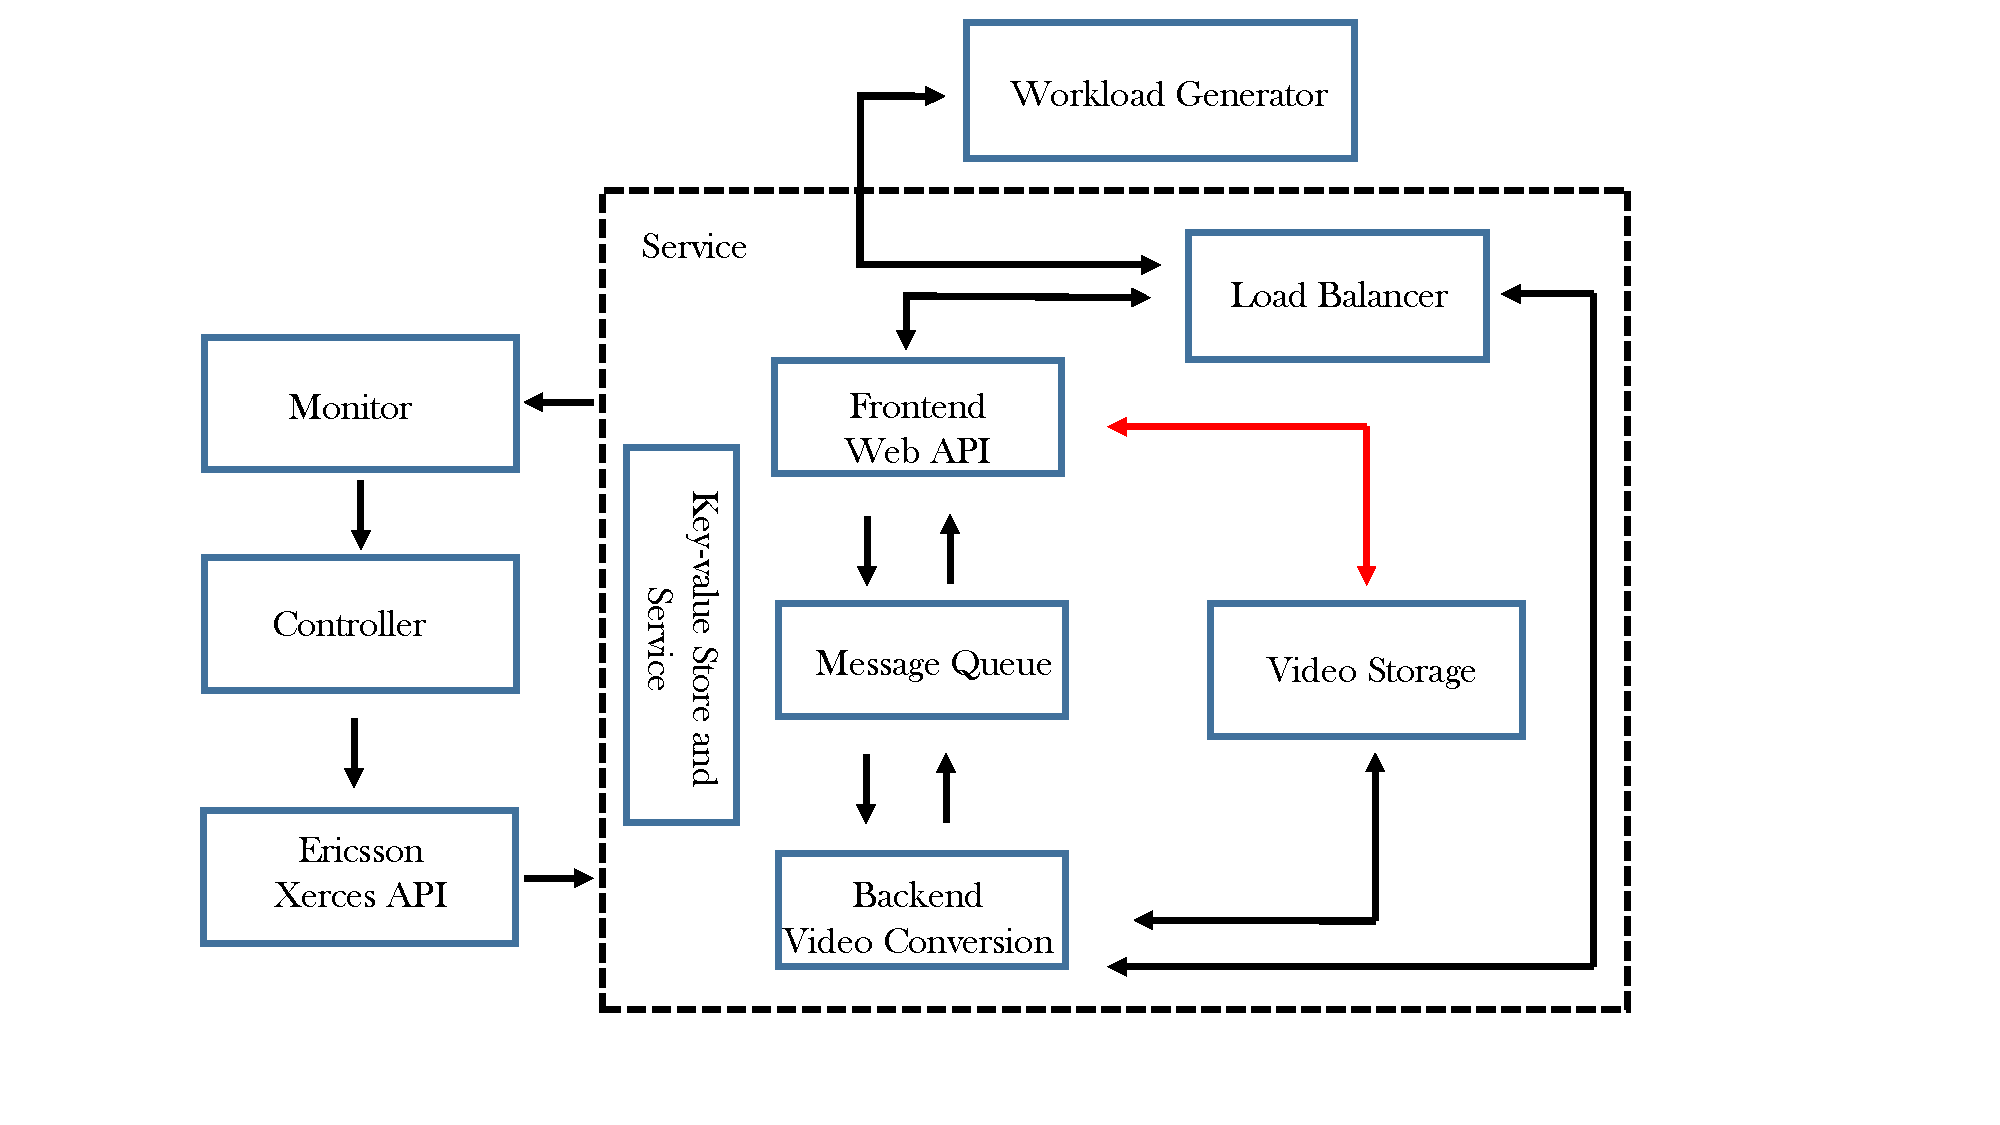
\includegraphics[width=1\textwidth]{figs/workflow.pdf}
	\caption{Overview of the system architecture.}
\end{figure}
An overview of the system architecture can be found in Figure~\ref{fig:architecture}. The different components involved are:
\begin{itemize}
	\item \textbf{Workload generator}: Is used as a test engine to simulate external users. See Section~\ref{sec:WG} for more details.
	\item \textbf{Load balancer}: Was not implemented due to lack of time.
	\item \textbf{Frontend Web API}: Is used to receive requests from users and deliver a response. See Section~\ref{sec:FE} for more details.
	\item \textbf{Message queue}: Is used to route the requests to the available Video conversion nodes and maintain the request queue. 
	\item \textbf{Backend Video conversion}: Is used to do the actual conversion of videos by reading the video from the storage. See Section~\ref{sec:BE} for more details.
	\item \textbf{Video Storage}: Is used to store available and converted videos.
	\item \textbf{Monitor}: Is be used to monitor entities relevant for the controller, by periodically gather information. The information is saved in .mat files, which can be used to plot the data in Matlab.
	\item \textbf{Controller}: Is used to make the service scalable. See Section~\ref{sec:Controller} for more details.
	\item \textbf{Health-Checking}: Is used to perform health checking for the backend and frontend nodes.
\end{itemize}

\section{Software and tech}
The following is a list of the software and tech that is used in the system components:
\begin{itemize}
	\item \textbf{Workload generator}: Python
	\item \textbf{Frontend Web API}: Python
	\item \textbf{Message queue}: RabbitMQ
	\item \textbf{Backend Video conversion}: FFmpeg with ffmpy
	\item \textbf{Video Storage}: Object storage in OpenStack
	\item \textbf{Monitor}: Python
	\item \textbf{Controller}: Python with python-novaclient (To interact with OpenStack).
	\item \textbf{Health-Checking}: Python with python-novaclient (To interact with OpenStack)
\end{itemize}

\section{Redundancy}
Due to lack of time, we were unable to implement redundancy in the components with states (such as the Message Queue and the Monitor).

\section{Workload generator} \label{sec:WG}
The workload generator is the test engine that simulates external users. It takes two parameters: the number of client converters and the average time between conversion requests. It starts the specified number of client threads, where each one represents a user. Each user randomly selects a video, sends a conversion request, waits for the completion, and then sleeps for a while (on average the specified time) before repeating the process.

The workload generator also measures the response time and stores it in a .mat-file.

\section{Frontend Web API} \label{sec:FE}
The Frontend Web API is used to receive requests from users and deliver a response. The conversion request is handled according to the following steps
\begin{itemize}
	\item The Frontend Web API receives a video conversion request, and sends this request to the Message Queue.
	\item Then, it waits for a response from the backend, which contains information of how to find the converted video in the storage.
	\item Finally, an "Accepted" response is sent to the user, where the information of how to find the converted video in the storage is included. If the backend does not accept the conversion request, an Error message is returned. 
\end{itemize}
When a user is requesting the actual converted video, the Frontend Web API checks if the converted video (which has a unique name) is available in the Video Storage using python-swiftclient. If it can be found, it responds with a OK message, otherwise an Error messasge is returned.


\section{Backend Video Conversion} \label{sec:BE}
The Backend Video Conversion node is used to perform the actual conversion of videos. When a conversion request is received from the Message Queue, the following steps are executed
\begin{itemize}
	\item First, the node checks if the requested video exists in the folder of available videos. If it does, the node sends an Accepted response back to the queue together with an unique file name, which represent where the converted file will be stored. Otherwise, an Error response is returned and the conversion is aborted. 
	\item The second step is to download the requested video from Video Storage and perform the actual conversion. For this, we used FFmpeg together with a Python wrapper called ffmpy.
	\item Finally, the converted file is uploaded to the Video Storage. Once this is done, the converted and downloaded videos are deleted locally.
\end{itemize}

\section{Controller} \label{sec:Controller}
The controller is used to scale up and down the number of VMs used for backend video conversion, depending on the workload. The controller is running at a frequency of 0.2 Hz

We used the simplifying assumption that all videos are of approximately the same size. This makes it possible to use the time from that a video conversion request is submitted until the video is converted as the control objective. Assume the average time it takes for one core to convert one video is given (including potential delays in the system), and denote it $ T_{\text{conv}} $. With $ n_{\text{queue}} $ video conversion requests in queue and $ n_{\text{vm}} $ active VMs, the time $ T $ needed to convert all videos in the queue is given by
\begin{equation}
T = \frac{T_{\text{conv}}  n_{\text{queue}}}{n_{\text{vm}}}
\end{equation}
Thus, if the control objective is to keep the maximum time from a request is submitted until the video is converted below $ T_{\text{max}} $, the number of VMs needed is given by
\begin{equation}
n_{\text{vm}} > \frac{T_{\text{conv}}  n_{\text{queue}}}{T_{\text{max}}}
\end{equation}

This is of course a simple approach which, if needed, could be extended to also consider videos of varying sizes and possibly reordering the queue such that for example small sized videos are prioritized over larger ones. By some simple tests, we got that $T_{\text{conv}} \approx 4$ seconds when we only had one request running at the time. We used $T_{\text{max}} = 12$ as the maximum , which gave us

\begin{equation*}
	r_{\text{vm}} = \text{max}\{n_{\text{lowest}}, \text{min}\{n_{\text{highest}}, \frac{T_{\text{conv}}  n_{\text{queue}}}{T_{\text{max}}}\} \}
\end{equation*} 
where $n_{\text{lowest}} = 2$ is the lowest amount of  active video conversion nodes, and $n_{\text{highest}} = 10$ is the highest amount of active video conversion nodes. 

To reduce the effect of quick, temporary  changes in the queue, we have used a low-passed filtered reference signal. We have also implemented a minimum time to live for the video conversion nodes, since the time from creation to actual work is long (currently couple of minutes, see FIGURE REF).

\section{Health-Checking} \label{sec:HC}
The Health-Checking node is used to make sure that the available Backend and Frontend nodes works. This is done by checking the Status flag in OpenStack. If a node has status Error, this node is deleted and then re-created again. This is done by using python Novaclient.


\section{Experimental Results}
Since we did not have time to implement the robustness for the system, the experimental evaluations were focused on scaling the service up and down depending on the workload. 


\end{document}
